\documentclass{article}
\usepackage[none]{hyphenat}
\usepackage{enumitem}
\usepackage{graphics}
\usepackage{graphicx}
\usepackage{listings}
\usepackage{ragged2e}
\usepackage{kvmap}
\usepackage{karnaugh-map}
\usepackage{multirow}
\usepackage[english]{babel}
\usepackage{caption}
\usepackage{tikz}
\usetikzlibrary{arrows,shapes,automata,petri,positioning,calc}

\title{SEQUENCE DETECTOR}
\date{March 2023}
\author{Lakkireddy Veerasiva Reddy\\lakkireddyveerasivareddy@gmail.com - FWC22122\\IIT Hyderabad-Future Wireless Communication}

\begin{document}

\maketitle
\tableofcontents
	\pagebreak
\section{Problem}
	(GATE EC-2020)\\
	Q.No.39. The state diagram of a sequence detector is shown below.State $S_0$ is the initial state of the sequence detector.If the output is 1,then
 \begin{figure}[h]
  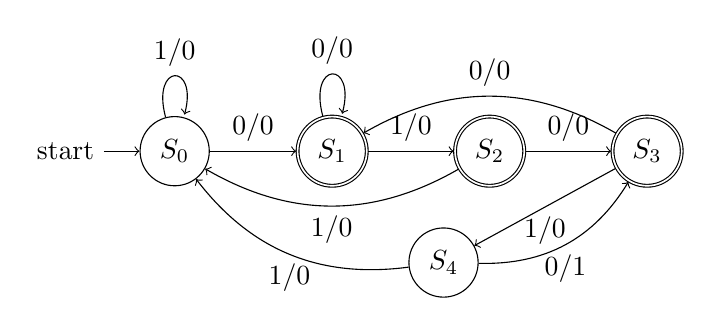
\begin{tikzpicture} [node distance=2cm]
\centering 
\node[circle, draw, state, initial] (S0) {$S_0$};
\node[circle, draw, state, accepting, right of=S0] (S1) {$S_1$};
\node[circle, draw, state, accepting, right of=S1] (S2) {$S_2$};
\node[circle, draw, state, accepting, right of=S2] (S3) {$S_3$}; 
\node[circle, draw, state, below right of = S1] (S4) {$S_4$};
\path[->] (S0) edge[above] node{0/0} (S1) 
          (S0) edge[loop above] node{1/0} (S0)
          (S1) edge[above] node{1/0} (S2)
          (S1) edge[loop above] node{0/0} (S1)
          (S2) edge[above] node{0/0} (S3) 
          (S2) edge[below,bend left] node{1/0} (S0)
          (S3) edge[below] node{1/0} (S4) 
          (S3) edge[above,bend right] node{0/0} (S1) 
          (S4) edge[below,bend left] node{1/0} (S0)   
          (S4) edge[below,bend right] node{0/1} (S3); 
\end{tikzpicture}

  \caption{State diagram}
  \label{fig:1}		
  \end{figure}	 
\begin{enumerate}
 \item the sequence 01010 is detected
 \item the sequence 01011 is detected
 \item the sequence 01110 is detected
 \item the sequence 01001 is detected	 
\end{enumerate}	
\section{Introduction}
  A sequence detector accepts as input a string of bits: either 0 or 1. Its output goes to 1 when a target sequence has been detected.There are two basic types:  overlap  and  non-overlap. In a sequence detector that allows overlap, the final bits of one sequence can be  the start of another sequence.
	\section{Components}	
\begin{table}[h]
\centering

\begin{tabular}{|c|c|c|}
\hline
Components & Value & Quantity\\
\hline
Resistor & 220 Ohm & 1\\
\hline
Arduino & UNO & 1\\
\hline
Seven Segment Display & & 1\\
\hline
Decoder & 7447 & 1\\
\hline
Flip Flop & 7474 & 2\\
\hline
Bread Board & & 1\\
\hline
Jumper Wires & & 20\\
\hline
\end{tabular}

\vspace{2mm}
\label{table:1}
\end{table}
\vspace{5mm}
\section{State Table}
  From state diagram,state table can be generated in Table 1.
  
  \vspace{5mm}
  \begin{table}[h]
  \centering
  \begin{tabular}{|c|c|c|c|}
  \hline
   
   \textbf{Present State}&{Input}&{Next state}&{Output}\\
   \hline
   
	 \textbf{$S_0$}&{0}&{$S_1$}&{0}\\
         \textbf{$S_0$}&{1}&{$S_0$}&{0}\\
         \textbf{$S_1$}&{0}&{$S_1$}&{0}\\
         \textbf{$S_1$}&{1}&{$S_2$}&{0}\\
         \textbf{$S_2$}&{0}&{$S_3$}&{0}\\
         \textbf{$S_2$}&{1}&{$S_0$}&{0}\\
         \textbf{$S_3$}&{0}&{$S_1$}&{0}\\
         \textbf{$S_3$}&{1}&{$S_4$}&{0}\\
         \textbf{$S_4$}&{0}&{$S_3$}&{1}\\
         \textbf{$S_4$}&{1}&{$S_0$}&{0}\\
  \hline
  \end{tabular}
  \vspace{5mm}
  \caption{State Table}  
  \end{table}

\subsection{Truth Table}
  
  \vspace{5mm}
  \begin{table}[h]
  \centering
  \begin{tabular}{|c|c|c|c|}
  \hline
   
   \textbf{Present State}&{Input}&{Next state}&{Output}\\
   \hline
   \textbf{A B C}&{X}&{P Q R}&{Y}\\
   \hline	  
   \textbf{0 0 0}&{0}&{0 0 1}&{0}\\
   \textbf{0 0 0}&{1}&{0 0 0}&{0}\\
   \textbf{0 0 1}&{0}&{0 0 1}&{0}\\
   \textbf{0 0 1}&{1}&{0 1 0}&{0}\\
   \textbf{0 1 0}&{0}&{0 1 1}&{0}\\
   \textbf{0 1 0}&{1}&{0 0 0}&{0}\\
   \textbf{0 1 1}&{0}&{0 0 1}&{0}\\
   \textbf{0 1 1}&{1}&{1 0 0}&{0}\\
   \textbf{1 0 0}&{0}&{0 1 1}&{1}\\
   \textbf{1 0 0}&{1}&{0 0 0}&{0}\\
  \hline
  \end{tabular}
  \vspace{5mm}
  \caption{Truth Table}
  \label{Table:2}
  \end{table}

\newpage
\section{Karnaugh Map}
  The karnaugh maps for the above truth table are given below

 \vspace{5mm}

\begin{karnaugh-map}[4][4][1][$CX$][$AB$]
	\minterms{7}
	\maxterms{0,1,2,3,4,5,6,8,9}
	\autoterms[$X$]
        \implicant{7}{15} 

    \end{karnaugh-map}
    \newline                                         
    \begin{equation}                                   P=BCX      
    \label{eq1}                
    \end{equation}

    \begin{karnaugh-map}[4][4][1][$CX$][$AB$]  
	    \minterms{3,4,8} 
	    \maxterms{0,1,2,5,6,7,9} 
	     \autoterms[$X$]
	       \implicant{4}{12}
	    \implicantedge{3}{3}{11}{11}
	    \implicantedge{12}{8}{14}{10}
	    
	    \end{karnaugh-map}   
	    \newline  
	    \begin{equation}   
	    Q = BC'X'+B'CX+AX'     
	      \label{eq2}   
	    \end{equation}

	\begin{karnaugh-map}[4][4][1][$CX$][$AB$]
		\minterms{0,2,4,6,8}     
	\maxterms{1,3,5,7,9}  
	\autoterms[$X$]
		\implicantedge{0}{8}{2}{10}
		\end{karnaugh-map}    
		\newline       
		\begin{equation}    
		R = X'   
		\label{eq3}    
		\end{equation}  

	\begin{karnaugh-map}[4][4][1][$CX$][$AB$]
		\minterms{8}   
		\maxterms{0,1,2,3,4,5,6,7,9}
		\autoterms[$X$]
		\implicantedge{12}{8}{14}{10}
		\end{karnaugh-map} 
		\newline         
		\begin{equation}  
		Y = AX'
		\label{eq4}     
		\end{equation}
\newpage
\section{Connections}
Connect the Arduino, 7447 ,two 7474 ICs and seven segment according to table 3.
\newline
{
\begin{table}[h]	
\centering
\scalebox{0.8}{
\begin{tabular}{|l|llll|llll|ll|llll|}
\hline
\multirow{2}{*}{} & \multicolumn{4}{l|}{INPUT}                                                    & \multicolumn{4}{l|}{OUTPUT}                                                   & \multicolumn{2}{l|}{}            & \multicolumn{4}{l|}{\multirow{2}{*}{5V}}                                       \\ \cline{2-11}
                  & \multicolumn{1}{l|}{A} & \multicolumn{1}{l|}{B} & \multicolumn{1}{l|}{C} & X  & \multicolumn{1}{l|}{P} & \multicolumn{1}{l|}{Q}  & \multicolumn{1}{l|}{R} & Y & \multicolumn{2}{l|}{CLOCK}       & \multicolumn{4}{l|}{}                                                          \\ \hline
Arduino           & \multicolumn{1}{l|}{6} & \multicolumn{1}{l|}{7} & \multicolumn{1}{l|}{8} & 9 & \multicolumn{1}{l|}{2} & \multicolumn{1}{l|}{3}  & \multicolumn{1}{l|}{4} & 5 & \multicolumn{2}{c|}{13}          & \multicolumn{1}{l|}{}  & \multicolumn{1}{l|}{}  & \multicolumn{1}{l|}{}   &    \\ \hline
7474              & \multicolumn{1}{l|}{5} & \multicolumn{1}{l|}{9} & \multicolumn{1}{l|}{}  &    & \multicolumn{1}{l|}{2} & \multicolumn{1}{l|}{12} & \multicolumn{1}{l|}{}  &   & \multicolumn{1}{l|}{CLK1} & CLK2 & \multicolumn{1}{l|}{1} & \multicolumn{1}{l|}{4} & \multicolumn{1}{l|}{10} & 13 \\ \hline
7474              & \multicolumn{1}{l|}{}  & \multicolumn{1}{l|}{}  & \multicolumn{1}{l|}{5} &    & \multicolumn{1}{l|}{}  & \multicolumn{1}{l|}{}   & \multicolumn{1}{l|}{2} &   & \multicolumn{1}{l|}{CLK1} & CLK2 & \multicolumn{1}{l|}{1} & \multicolumn{1}{l|}{4} & \multicolumn{1}{l|}{10} & 13 \\ \hline
	7447              & \multicolumn{1}{l|}{} & \multicolumn{1}{l|}{} & \multicolumn{1}{l|}{} &    & \multicolumn{1}{l|}{7}  & \multicolumn{1}{l|}{1}   & \multicolumn{1}{l|}{2}  & 6  & \multicolumn{1}{l|}{} &   & 16 &  \\ \hline
\end{tabular}
}

 \vspace{3mm}
  \caption{Connection Table}
  \label{Table:3}	
  \end{table}
 \vspace{5mm} 
\section{Software}
The arduino code for the given sequence detector is given below \\

   \lstinputlisting{gate2020.cpp}

\end{document}
